% Autogenerated translation of README.md by Texpad
% To stop this file being overwritten during the typeset process, please move or remove this header

\documentclass[12pt]{book}
\usepackage{graphicx}
\usepackage{fontspec}
\usepackage[utf8]{inputenc}
\usepackage[a4paper,left=.5in,right=.5in,top=.3in,bottom=0.3in]{geometry}
\setlength\parindent{0pt}
\setlength{\parskip}{\baselineskip}
\setmainfont{Helvetica Neue}
\usepackage{hyperref}
\pagestyle{plain}
\begin{document}

\chapter*{STN Scheduler}

The State-Task Network (STN) is a method for modeling and scheduling multipurpose batch processes developed by Kondili, et al., in 1993, and extended by others. 

This repository consists of a python module STN to assist in the modeling and scheduling of State Task Networks, and Jupyter notebooks demonstrating their use. 

\begin{itemize}
\item \href{http://nbviewer.jupyter.org/github/jckantor/STN-Scheduler/blob/master/notebooks/0_Overview.ipynb}{Overview of STN Scheduler (to be finished)}
\item \href{http://nbviewer.jupyter.org/github/jckantor/STN-Scheduler/blob/master/notebooks/1_Kondili_State_Task_Network.ipynb}{State Task Network Example of Kondili, et. al, 1993}.
\item \href{http://nbviewer.jupyter.org/github/jckantor/STN-Scheduler/blob/master/notebooks/2_Chu_State_Task_Network.ipynb}{State Task Network Example of Chu, et. al, 2013}.
\item \href{http://nbviewer.jupyter.org/github/jckantor/STN-Scheduler/blob/master/notebooks/4_Maravelias_Grossmann_Example_A.ipynb}{Example from Maravelias and Grossmann, 2003}.
\item \href{http://nbviewer.jupyter.org/github/jckantor/STN-Scheduler/blob/master/notebooks/3_Multipurpose_Fermentation_Plant.ipynb}{Classroom Case Study of a Multipurpose Batch Fermentation Plant (to be finished)}.
\end{itemize}

This module implements the STN model using the Pyomo package for building optimization models in \href{http://www.pyomo.org/}{Python}, and requires an MILP solver to compute schedules.

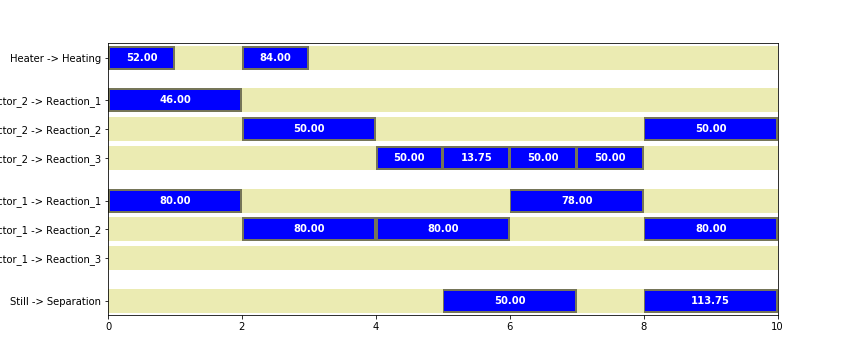
\includegraphics{images/Kondili_gantt.png}

\section*{Dependencies}

\begin{itemize}
\item \href{http://www.pyomo.org/}{Pyomo}
\item An MILP solver is required for computing solutions to the MILP scheduling problems. The module has been tested with GLPK and Gurobi.
\end{itemize}

\section*{Related Projects}

\begin{itemize}
\item \href{https://github.com/robin-vjc/pySTN}{pySTN} Implementation of a robust scheduling system based on STN (State-Task-Network) models.
\end{itemize}

\end{document}
